\subsubsection{Estimating our preferred model}\label{LESresults}
Based on the criteria described in the previous section, we proceed with model 7 as our preferred model. We estimate the model on 6 different datasets, 5 for each quintile of the distribution of disposable income (which we will refer to as simply 'the income distribution', and 1 for the average household. 
Recall the we model consumer demand as
\begin{align}
    p_{it} x_{it} = p_{it} b_{it} + \alpha_i(\mu - \sum p_{kt} b_{kt}),
\end{align}
where
\begin{align} \label{eq:habitform}
    b_{it} = \beta_{1i} x_{i,t-1} + \beta_{2i} b_{i,t-1}.
\end{align}

In table \ref{mdl7estpart1} we see that the model fits best on the average household. This is most likely due to the average household having a more smoothed series, as can be seen from [insert reference to relevant figure]. The likelihood of the model fitted to average household data is 799, compared to likelihoods in the range 689-744 for the different quintiles. Obviously, as the number of the parameters and the sample size is the same across datasets, the higher likelihood also results in a higher BIC. 

Recall that the marginal budget share, $\alpha$, is defined by
\begin{equation}
    \alpha= \frac{\partial p_i x_i}{\partial \mu},
\end{equation}
that is, the change in expenditure on a given good with respect to a change in total expenditure. Generally speaking, the estimated marginal budget shares are not very different across the income distribution. From our bootstrapped standard errors, we see that few estimates are significantly different across the income distribution, with an exception to the rule being the marginal budget share of meat and dairy for quintile 1 and 2. 

The marginal budget share of meat and dairy is in around .03 for all quintiles except the first. For other foods, it is in the range .03-.08, but with no clear gradient across the income distribution. For housing, the estimate is in the range .10-.13 for all quintiles.

Energy for housing, where we ex-ante would expect marginal budget shares to differ, as the poorer households have a larger consumption share of this good composite than the rich households. As is obvious from table  \ref{mdl7estpart1}, there is no clear cut relationship between the marginal budget share and income for energy for housing. However, both quintile 4 and 5 have lower estimates than the average. For energy for transport, we see what potentially could be an income gradient in the marginal budget share for energy for transport - the richer households tend to have a lower marginal budget share. For transport goods and services, which include the purchase of cars, there is no clear relationship. All estimates lie in the range 0.20-0.28. For other goods, there seems to be a U-shaped relationship between the marginal budget share and income.  However, the highest marginal budget share is estimated for the average household. For other services, there could be an indication a positive income gradient, that is, the higher income, the larger marginal budget share.

\begin{table}[H]
\renewcommand{\arraystretch}{0.7}
\centering
\caption{Estimation results, part 1}
\label{mdl7estpart1}
\begin{tabular}{lcccccc}
  \multicolumn{7}{c}{Model information} \\\hline
Quintile & 1 & 2 & 3 & 4 & 5 & Avg. \\ 
  \hline
Likelihood & -689.43 & -723.17 & -713.13 & -743.48 & -733.04 & -799.60 \\ 
  BIC & -1214.70 & -1282.19 & -1262.11 & -1322.80 & -1301.91 & -1435.04 \\ 
   \hline \\
\multicolumn{7}{c}{Estimates of $\alpha$} \\ 
  \hline
 Quintile & 1 & 2 & 3 & 4 & 5 & Avg. \\ 
  \hline
Meat.and.dairy & 0.008 & 0.039 & 0.034 & 0.034 & 0.029 & 0.028 \\ 
 & (0.014) & (0.008) & (0.012) & (0.011) & (0.007) & (0.007) \\ 
  Other.foods & 0.032 & 0.081 & 0.067 & 0.078 & 0.037 & 0.036 \\ 
   & (0.029) & (0.019) & (0.021) & (0.021) & (0.024) & (0.02) \\ 
  Housing & 0.131 & 0.104 & 0.122 & 0.138 & 0.11 & 0.072 \\ 
   & (0.03) & (0.037) & (0.033) & (0.028) & (0.033) & (0.026) \\ 
  Energy.for.housing & 0.105 & 0.029 & 0.122 & 0.077 & 0.068 & 0.112 \\ 
  & (0.02) & (0.023) & (0.021) & (0.013) & (0.01) & (0.021) \\ 
  Energy.for.transport & 0.03 & 0.025 & 0.025 & 0.025 & 0.018 & 0.03 \\ 
   & (0.013) & (0.008) & (0.008) & (0.01) & (0.007) & (0.007) \\ 
  Transport & 0.231 & 0.276 & 0.244 & 0.265 & 0.207 & 0.241 \\ 
   & (0.039) & (0.045) & (0.045) & (0.048) & (0.024) & (0.033) \\ 
  Other.goods & 0.291 & 0.244 & 0.169 & 0.199 & 0.286 & 0.293 \\ 
& (0.051) & (0.041) & (0.051) & (0.047) & (0.05) & (0.038) \\ 
  Other.services & 0.172 & 0.202 & 0.217 & 0.183 & 0.244 & 0.188 \\ 
 & (0.048) & (0.051) & (0.054) & (0.05) & (0.029) & (0.037) \\ \hline

\end{tabular}


\captionsetup{singlelinecheck=off,size=scriptsize}
\setlength{\captionmargin}{10pt}
\caption*{
\textbf{Note:} Standard errors in parentheses}
\end{table}
The estimates of $\beta_1$ and $\beta_2$ are difficult to interpret by themselves. Together, they model the habit formation as described in equation (\ref{eq:habitform}). In table \ref{mdl7estpart2}, where these estimates are reported, it seems that there is a clear tendency for $\beta_1+\beta_2$ to be close to 1 for many goods. For almost all goods and quintiles, $\beta_1>\beta_2$, indicating that the most important part of habit formation is not past minimum consumption, but rather past consumption. 

\begin{table}[H]
\centering
\renewcommand{\arraystretch}{0.7}
\caption{Estimation results, part 2}
\label{mdl7estpart2}
\begin{tabular}{lcccccc}

\multicolumn{7}{c}{Estimates of $\beta_1$} \\ 
  \hline
Quintile & 1 & 2 & 3 & 4 & 5 & Avg. \\ 
  \hline
Meat.and.dairy & 0.873 & 0.838 & 0.725 & 0.792 & 0.671 & 0.806 \\ 
   & (0.201) & (0.175) & (0.184) & (0.201) & (0.156) & (0.081) \\ 
  Other.foods & 0.842 & 0.925 & 0.842 & 0.807 & 0.847 & 0.91 \\ 
   & (0.18) & (0.158) & (0.11) & (0.171) & (0.189) & (0.129) \\ 
  Housing & 0.461 & 0.84 & 0.608 & 0.724 & 0.796 & 0.86 \\ 
   & (0.124) & (0.201) & (0.164) & (0.174) & (0.153) & (0.177) \\ 
  Energy.for.housing & 0.109 & 1.024 & 0.116 & 0.346 & 0.169 & 0.084 \\ 
   & (0.126) & (0.272) & (0.125) & (0.089) & (0.127) & (0.133) \\ 
  Energy.for.transport & 1.096 & 0.989 & 0.692 & 0.761 & 0.564 & 0.6 \\ 
   & (0.146) & (0.173) & (0.153) & (0.186) & (0.209) & (0.133) \\ 
  Transport & 0.701 & 0.28 & 0.624 & 0.53 & 0.047 & 0.301 \\ 
   & (0.194) & (0.094) & (0.256) & (0.19) & (0.092) & (0.127) \\ 
  Other.goods & 0.778 & 1.062 & 0.983 & 0.904 & 0.477 & 0.951 \\ 
   & (0.16) & (0.188) & (0.239) & (0.197) & (0.184) & (0.131) \\ 
  Other.services & 0.691 & 0.803 & 0.669 & 0.679 & 0.467 & 0.699 \\ 
   & (0.234) & (0.25) & (0.252) & (0.202) & (0.138) & (0.178) \\
   \hline\\
\multicolumn{7}{c}{Estimates of $\beta_2$} \\ 
   \hline
Quintile & 1 & 2 & 3 & 4 & 5 & Avg. \\ 
  \hline
Meat.and.dairy & 0.089 & 0.095 & 0.17 & 0.103 & 0.152 & 0.091 \\ 
   & (0.228) & (0.188) & (0.212) & (0.239) & (0.17) & (0.073) \\ 
  Other.foods & 0.095 & -0.007 & 0.031 & 0.068 & 0.025 & 0.014 \\ 
   & (0.192) & (0.157) & (0.115) & (0.203) & (0.214) & (0.12) \\ 
  Housing & 0.486 & 0.123 & 0.329 & 0.199 & 0.076 & 0.09 \\ 
   & (0.128) & (0.235) & (0.191) & (0.185) & (0.165) & (0.18) \\ 
  Energy.for.housing & 0.863 & -0.059 & 0.846 & 0.585 & 0.758 & 0.892 \\ 
   & (0.134) & (0.328) & (0.193) & (0.102) & (0.17) & (0.144) \\ 
  Energy.for.transport & -0.484 & -0.099 & 0.172 & 0.128 & 0.306 & 0.25 \\ 
   & (0.274) & (0.207) & (0.17) & (0.194) & (0.26) & (0.136) \\ 
  Transport & -0.73 & 0.611 & -0.086 & 0.182 & 0.92 & 0.495 \\ 
   & (0.43) & (0.236) & (0.413) & (0.351) & (0.146) & (0.242) \\ 
  Other.goods & -0.17 & -0.22 & -0.183 & -0.078 & 0.198 & -0.338 \\ 
   & (0.303) & (0.225) & (0.254) & (0.215) & (0.292) & (0.183) \\ 
  Other.services & 0.155 & 0.122 & 0.189 & 0.229 & 0.324 & 0.172 \\ 
   & (0.262) & (0.262) & (0.305) & (0.217) & (0.173) & (0.196) \\ 
   \hline
\end{tabular}
\captionsetup{singlelinecheck=off,size=scriptsize}
\setlength{\captionmargin}{10pt}
\caption*{
\textbf{Note:} Standard errors in parentheses}
\end{table}

To grasp what the estimates for $\beta_1$ and $\beta_2$ imply for the minimum consumption levels, these are plotted in figure  \ref{fig:mincons}. One feature of the minimum consumption levels, e.g. for meat and dairy as well as other foods, is that minimum consumption are much closer to actual consumption for the poorer quintiles compared to the richer quintiles. This is in accordance with our expectations. Poor households and rich households most likely \textit{need} the same amount of food, and thus minimum consumption should be closer to actual consumption for the poorer households. The result also makes intuitive sense considering Engels' law. As poorer households spend a larger share out of total expenditure on food, it makes sense that their minimum consumption levels are closer to actual consumption. 

For housing, minimum consumption follows actual consumption quite closely. It seems plausible that habit formation is strong for housing, as there are high costs to moving. Regarding energy for housing we see that the minimum consumption levels of the middle and the richest quintile are quite close, but lower for the bottom quintile. This indicates that the relationship between income and necessary expenditure on energy for housing is concave. The difference in energy for housing minimum consumption needs can most likely also be explained by poorer households having smaller dwellings to heat and perhaps fewer electric appliances.

The minimum consumption needs for energy for transport also differ a lot across the income distribution. Common to all of them are that they are pretty close to actual consumption, indicating that is a necessity good. The transport good and service composite seems to be more of a luxury good. Minimum consumptions is further below actual consumption for all 3 quintiles graphed. 

Finally, the broader good composites other goods and other services seem described a bit more as luxury goods, which is as expected. Minimum consumption levels, especially for the richest households, are quite far off actual consumption. 

\begin{figure}[H]
\centering
\caption{Minimum consumption and actual consumption for different quintiles}
\label{fig:mincons}
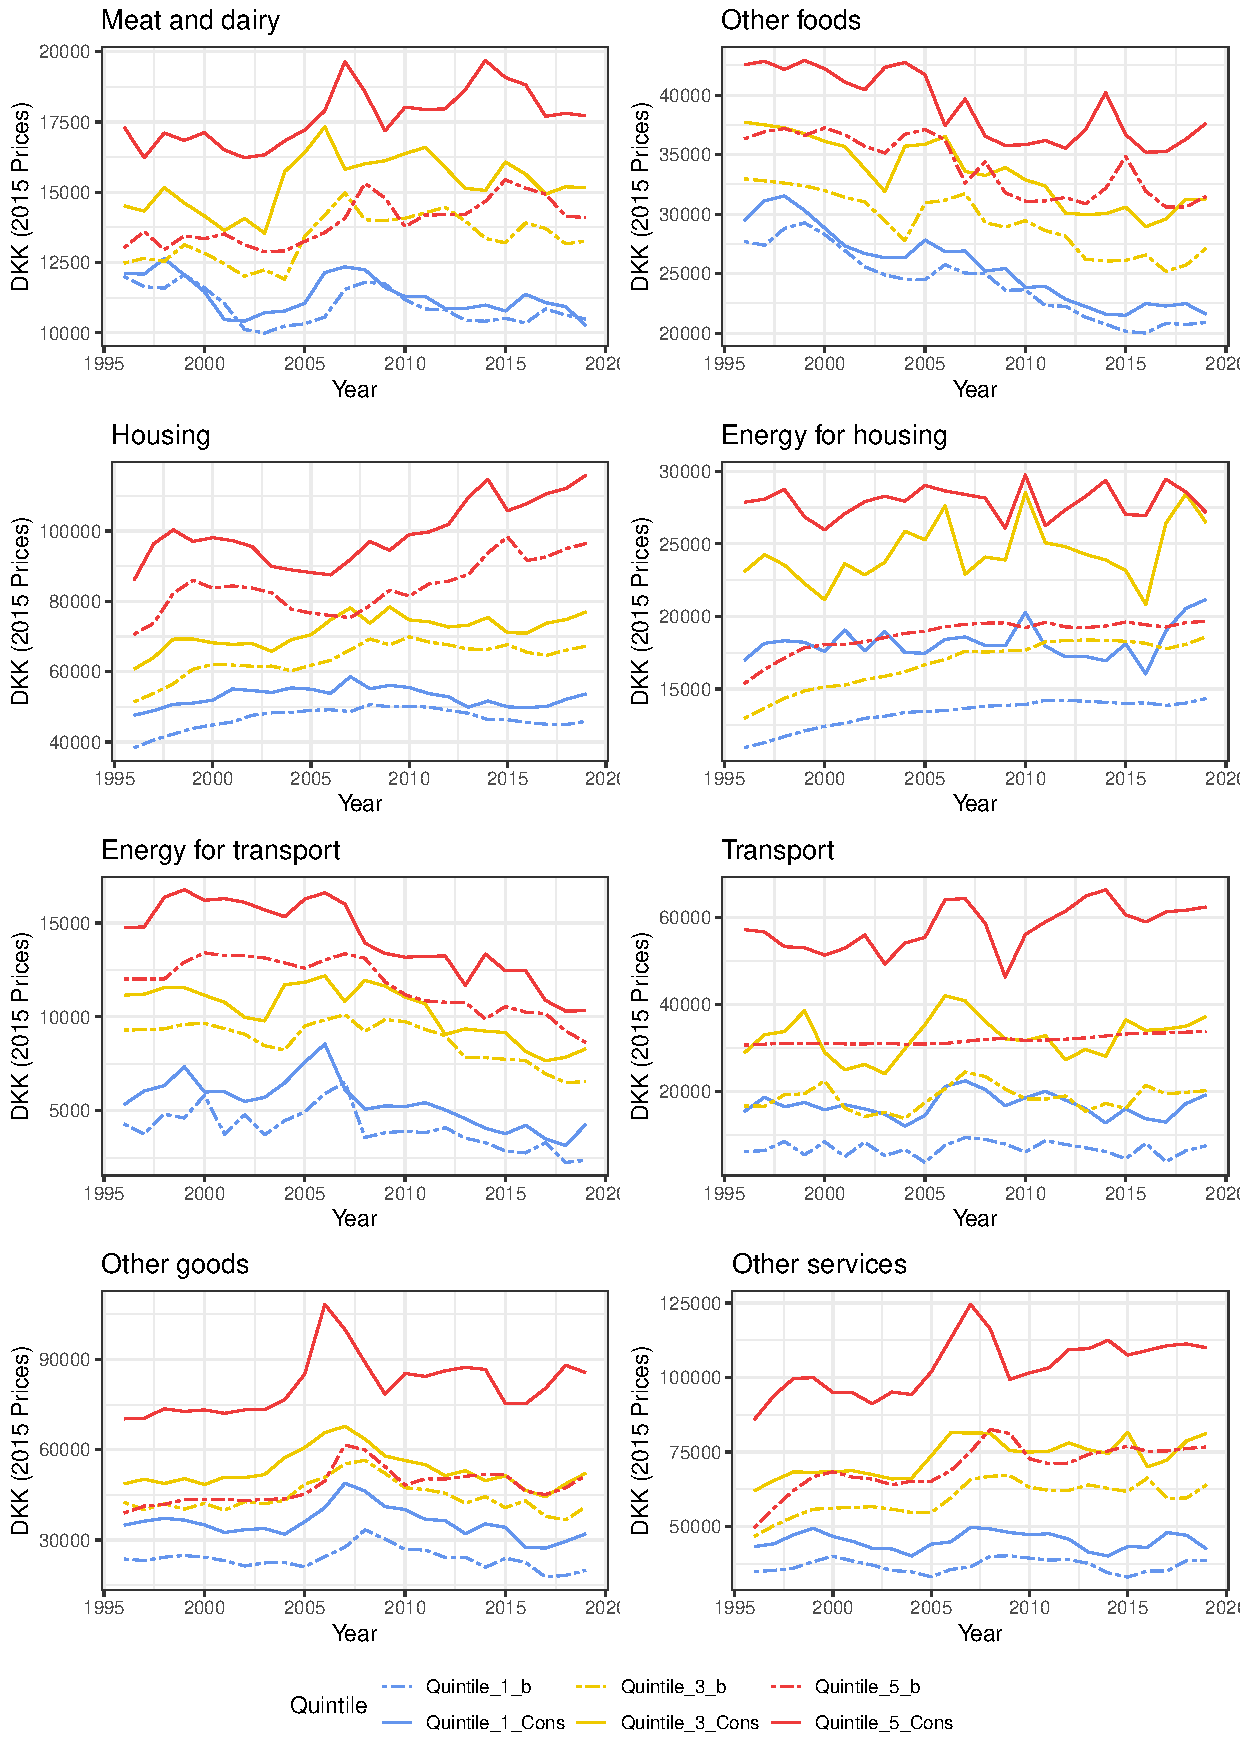
\includegraphics[width=.9\textwidth]{Figures/b_quintileplot.pdf}
\captionsetup{singlelinecheck=off,size=scriptsize}
\setlength{\captionmargin}{10pt}
\caption*{
\textbf{Note:} Solid lines indicate actual consumption in 2015-prices. Dashed lines indicate minimum consumption levels.\\}
\end{figure}

\begin{table}[H]
\centering
\renewcommand{\arraystretch}{0.7}
\caption{Estimation results, minimum consumption levels}
\label{mdl7estpart}
\begin{tabular}{rllllll}
  \multicolumn{7}{c}{Estimates of $b$, minimum consumption levels, 2019} \\ 
  \hline
 & 1 & 2 & 3 & 4 & 5 & Avg. \\ 
  \hline
Meat.and.dairy & 10488.773 & 11714.424 & 13257.823 & 15225.205 & 14099.277 & 12963.745 \\ 
   & (36.669) & (24.823) & (44.972) & (42.7) & (32.85) & (22.536) \\ 
  Other.foods & 20887.35 & 23749.634 & 27114.018 & 29519.344 & 31489.343 & 27413.937 \\ 
   & (61.629) & (76.931) & (83.608) & (55.615) & (129.481) & (56.773) \\ 
  Housing & 45916.011 & 57694.225 & 67257.615 & 74282.764 & 96410.321 & 71469.5 \\ 
   & (73.542) & (148.447) & (123.774) & (169.488) & (298.584) & (118.687) \\ 
  Energy.for.housing & 14351.331 & 21008.824 & 18588.465 & 21403.008 & 19660.7 & 18005.982 \\ 
   & (23.689) & (160.748) & (29.619) & (53.406) & (32.785) & (19.973) \\ 
  Energy.for.transport & 2354.806 & 5000.434 & 6546.01 & 8683.687 & 8641.662 & 5804.662 \\ 
   & (93.6) & (39.24) & (42.858) & (42.056) & (45.443) & (25.348) \\ 
  Transport & 7430.79 & 15030.98 & 20102.423 & 32129.377 & 33766.149 & 21011.24 \\ 
   & (153.068) & (69.633) & (140.155) & (132.843) & (54.243) & (58.344) \\ 
  Other.goods & 19875.455 & 35909.046 & 41078.755 & 48987.765 & 51432.483 & 38146.995 \\ 
   & (172.791) & (236.82) & (258.436) & (250.414) & (243.954) & (217.266) \\ 
  Other.services & 38512.693 & 54078.335 & 64006.826 & 79241.798 & 76722.777 & 64143.2 \\ 
   & (149.297) & (118.286) & (172.093) & (152.143) & (165.571) & (114.237) \\ 
   \hline
\end{tabular}
\captionsetup{singlelinecheck=off,size=scriptsize}
\setlength{\captionmargin}{10pt}
\caption*{
\textbf{Note:} Standard errors in parentheses}
\end{table}


The low marginal budget share and high minimum consumption levels impliy that the own-price elasticity of meat and dairy and other foods are lower for the poorer quintiles. The income elasticities are also lower for the poorest quintiles for these two good composites, but rise with income. For the rest of the good composites, there is no clear relationship between own-price elasticities and income. Transport and other goods have the highest elasticities, while housing, other services and the two energy good compositse have way lower elasticities. 
\begin{table}[H]
\centering
\renewcommand{\arraystretch}{0.7}
\caption{Estimation results, part 3}
\label{mdl7estpart3}
\begin{tabular}{lcccccc}
\multicolumn{7}{c}{Estimates of own price elasticity} \\ 
  \hline
Quintile & 1 & 2 & 3 & 4 & 5 & Avg. \\ 
  \hline
Meat.and.dairy & -0.044 & -0.123 & -0.187 & -0.147 & -0.246 & -0.142 \\ 
   & (0.054) & (0.024) & (0.055) & (0.04) & (0.047) & (0.028) \\ 
  Other.foods & -0.097 & -0.165 & -0.214 & -0.203 & -0.174 & -0.11 \\ 
   & (0.063) & (0.037) & (0.057) & (0.043) & (0.085) & (0.051) \\ 
  Housing & -0.232 & -0.148 & -0.226 & -0.221 & -0.229 & -0.125 \\ 
   & (0.046) & (0.048) & (0.05) & (0.04) & (0.06) & (0.041) \\ 
  Energy.for.housing & -0.347 & -0.068 & -0.426 & -0.248 & -0.387 & -0.373 \\ 
   & (0.058) & (0.045) & (0.055) & (0.036) & (0.038) & (0.059) \\ 
  Energy.for.transport & -0.392 & -0.15 & -0.243 & -0.164 & -0.238 & -0.262 \\ 
   & (0.17) & (0.041) & (0.063) & (0.058) & (0.067) & (0.047) \\ 
  Transport & -0.694 & -0.534 & -0.61 & -0.51 & -0.577 & -0.562 \\ 
  & (0.092) & (0.076) & (0.067) & (0.069) & (0.04) & (0.051) \\ 
  Other.goods & -0.597 & -0.378 & -0.378 & -0.364 & -0.613 & -0.535 \\ 
   & (0.062) & (0.051) & (0.087) & (0.069) & (0.057) & (0.047) \\ 
  Other.services & -0.316 & -0.28 & -0.375 & -0.28 & -0.475 & -0.312 \\ 
   & (0.069) & (0.065) & (0.076) & (0.064) & (0.042) & (0.052) \\ 
   \hline\\
\multicolumn{7}{c}{Estimates of expenditure elasticity} \\ 
   \hline
Quintile & 1 & 2 & 3 & 4 & 5 & Avg. \\ 
  \hline
Meat.and.dairy & 0.154 & 0.739 & 0.686 & 0.71 & 0.737 & 0.59 \\ 
   & (0.194) & (0.139) & (0.199) & (0.195) & (0.141) & (0.118) \\ 
  Other.foods & 0.286 & 0.765 & 0.678 & 0.824 & 0.469 & 0.384 \\ 
   & (0.193) & (0.174) & (0.181) & (0.175) & (0.229) & (0.179) \\ 
  Housing & 0.496 & 0.411 & 0.508 & 0.586 & 0.443 & 0.288 \\ 
   & (0.101) & (0.131) & (0.112) & (0.108) & (0.115) & (0.096) \\ 
  Energy.for.housing & 1.152 & 0.345 & 1.494 & 1.128 & 1.129 & 1.475 \\ 
   & (0.188) & (0.212) & (0.192) & (0.165) & (0.111) & (0.229) \\ 
  Energy.for.transport & 1.588 & 1.072 & 0.964 & 0.866 & 0.741 & 1.204 \\ 
   & (0.741) & (0.28) & (0.247) & (0.31) & (0.206) & (0.208) \\ 
  Transport & 2.565 & 2.993 & 2.087 & 2.026 & 1.543 & 2.126 \\ 
   & (0.347) & (0.394) & (0.227) & (0.281) & (0.104) & (0.189) \\ 
  Other.goods & 1.834 & 1.495 & 1.086 & 1.255 & 1.514 & 1.721 \\ 
   & (0.195) & (0.2) & (0.253) & (0.227) & (0.145) & (0.148) \\ 
  Other.services & 0.739 & 0.821 & 0.87 & 0.722 & 1.008 & 0.767 \\ 
   & (0.167) & (0.195) & (0.181) & (0.165) & (0.091) & (0.131) \\ 
   \hline
\end{tabular}
\captionsetup{singlelinecheck=off,size=scriptsize}
\setlength{\captionmargin}{10pt}
\caption*{
\textbf{Note:} Standard errors in parentheses}
\end{table}
The expenditure elasticities of energy for transport are decreasing across the income distribution. As expenditure rises, the poorer quintiles will tend to increase their consumption of this good relatively more than the richer households. The same can be said for the transport good composite. At the same time, these two goods have the highest expenditure elasticities, indicating that these are luxury goods, but more so for the lower quintiles.


\subsection{Endogeneity concerns}
A possible cause of endogenity is the fact that we do not model the choice between savings and consumption. Total expenditure is treated as if it was disposable income. An increase in total expenditure will, for unchanged $b$, result in increased consumption of each of the $n=8$ goods with their respective marginal budget share $\alpha_i$, where $\sum \alpha_i=1$. An increase in disposable income will, in reality, most likely increase both total expenditure and savings. 

One potential source of endogeneity in our models is the fact that price increases cannot affect savings. Consider our estimation equation
\begin{align}
    w_{it} = \frac{p_{it} b_{it}}{\mu_t} + \alpha_i \left( 1-\frac{\sum p_{kt}b_{kt}}{\mu_t}\right)+ u_{it}.
\end{align}
Let us assume that the price of a specific good which has a high level of minimum consumption $b$. If the price of that increases significantly, in our model, it only affects the consumption of other goods. In reality, the consumer may choose to lower her savings, increasing total expenditure (an income effect). On the other hand, increased prices for relatively unimportant goods, may lead the consumer to increase savings, as consumption has become more expensive (a substitution effect). Thus the effect of prices on savings behaviour is ambigous, and the direction of potential bias of our estimates are uncertain.

The fact that we estimate our parameters on consumption \textit{shares} may mitigate the bias. If a price increase of a given good increases savings, total expenditure falls - and that will, all else equal, lower consumption of all goods by their marginal budget share. Thus, the consumption share, $w_{it}$, may be approximately unaffected. 
